%======================================================================
\chapter{Mechanism of \texorpdfstring{\ce{CO2}}{CO2} Reduction}\label{chap.mech}
\markright{Computational Study of the Mechanism of \texorpdfstring{\ce{CO2}}{CO2} Reduction}
%======================================================================

%======================================================================
\section{Introduction}
%======================================================================

Within three years of the appearance of the originally reported bipyridine rhenium (I) catalyst, experimental studies on the mechanism of the photocatalytic reduction of \ce{CO2} were available in the literature\autocite{hawecker1986}. Studies continue on the mechanism up to the present day\autocite{johnson1996, koike2002, takeda2008, smieja2012, machan2014, kou2014}, utilizing new investigative techniques as they become available to elucidate transition states and transient intermediates \textit{in situ}. 

The mechanistic studies performed analyze \ce{CO2} reduction both photocatalytically and electrocatalytically on Re compounds. The electrocatalytic activity was demonstrated by Hawecker \textit{et. al.} only a year after the photochemistry first appeared\autocite{hawecker1984}. Both methods involve similar cycles, and have been treated interchangeably by some authors\ref{authors}, the difference between methods being the production of the excimer species, not the first 2\textit{e}\textsuperscript{-} reduction at the active site. Electrochemical methods have been employed with the hope of utilizing \ce{CO2} and \ce{H2O} together for the direct formation of methane and oxygen\todo{ref}, this target remains elusive and is not within the scope of this study.

Investigation includes the use of \gls{ac.dft} methods to elucidate geometries of intermediates and transition states for of the multi-step cycle. Transition metal catalysis is a non-trivial problem computationally, particularly when considering a metal from the lower period. These elements contain a large amount of electrons, many of which can be involved in non-covalent interactions with the ligands and catalyzed products. Solving for this complex system becomes non-trivial and computationally expensive. For this reason, no overview of the mechanism as investigated by \gls{ac.dft} methods has ever been made available in the literature. 

%======================================================================
\section{Mechanism Pathways}
%======================================================================

Prior work in the literature has proposed three general mechanistic pathways for the photoreduction of \ce{CO2}. In general, as seen in \autoref{fig.threepath}, these pathways result in the formation of \ce{CO} and \ce{H2O}, formate (\ce{HCO2-}), or carbonate (\ce{CO3H-}) anions. The formation of carbonate proceeds via the formation of a catalyst dimer over a molecule of \ce{CO2}, with the insertion of a second molecule of \ce{CO2} to produce the carbonate and a molecule of \ce{CO}. Production of formate occurs via insertion of \ce{CO2} to a rhenium hydride bond. The formation of \ce{CO} without carbonate or formate by-products occurs via the coordination of \ce{CO2} to an open site on the metal, followed by a double proton addition and the release of a molecule of \ce{H2O} prior to the loss of one of the four carbonyl groups to open up the axial site for halide re-coordination. This is essentially the \gls{ac.rwgsr}, wherein protons are made available from decomposition of the sacrificial amine instead of from decomposition of \ce{H2}\autocite{kalyanasundaram1978}. These three mechanistic pathways will be referred to as the `carbonate' mechanism, the `formate' mechanism, and the `water-gas shift' mechanism, respectively.
\todo{Energy jumps at the disassociation steps may be due to the charge separation. Crunch numbers of Gibbs (when available) and try and work away from 100's of kcal values}

\begin{figure}[!htb]
 \begin{center}
  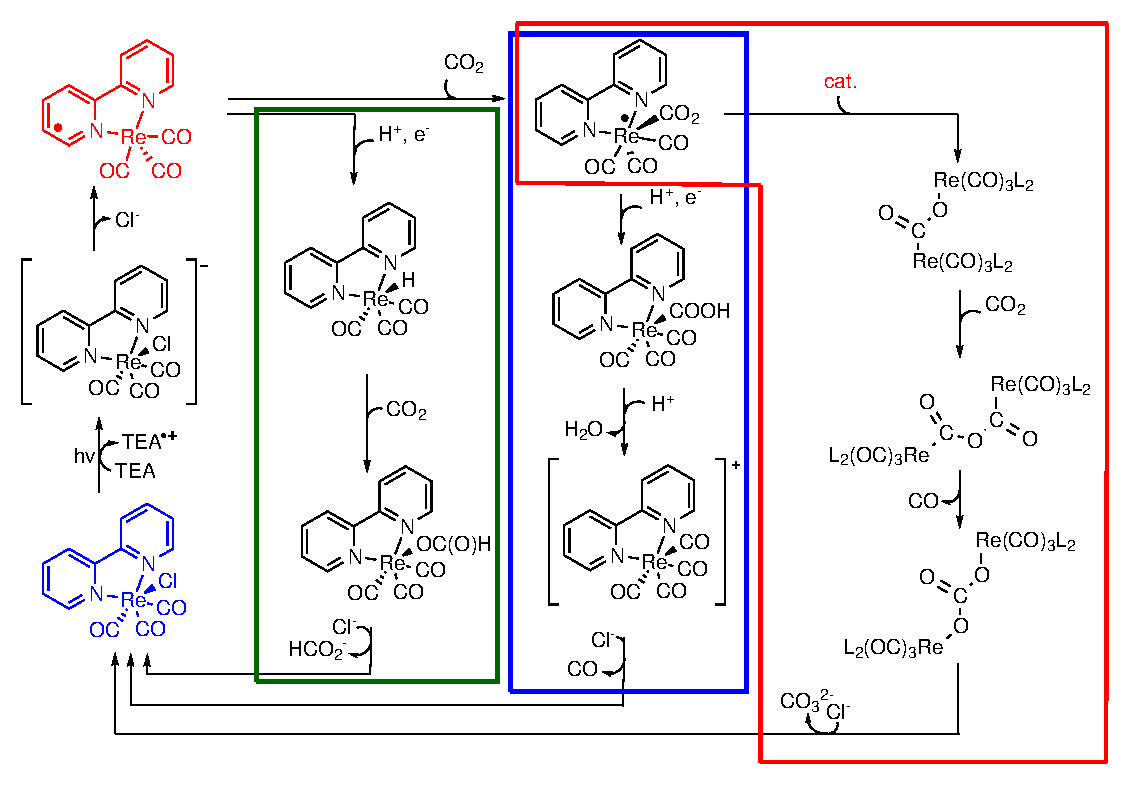
\includegraphics[clip=true, width=\textwidth, keepaspectratio]{images/threepaths.eps}
 \end{center}
\caption[Overview of mechanistic pathways]{An overview of the mechanistic pathways of photochemical \ce{CO2} reduction. Catalyst is shown in blue, and the excimer species in red}
\label{fig.threepath}
\end{figure} 

Each of the mechanistic pathways identified above in \autoref{fig.threepath} was studied, using \gls{ac.dft} methods. Structures (using 2,2'-bipyridine as the bidentate ligand, and triethylamine as the sacrificial reductant) were optimized to ground or transition states using TurboMole 6.5\autocite{turbomole, ahlrichs1989}, with the TPSS meta-GGA XC functional\autocite{tao2003}. The def2-TZVP basis set was used for all atoms\autocite{schafer1994, weigend2005}. The TurboMole program contains a number of optimizations to the original \gls{ac.dft} algorithms\autocite{haase1993, treutler1995, eichkorn1997, eichkorn1995, sierka2003, deglmann2004, weigend2002, vonarnim1998, ahlrichs2004}, decreasing the calculation time without compromising accuracy. Grimme's dispersion correction (version 3) was included in the calculations\autocite{grimme2010}. Intermediates and transition states were verified by frequency analysis\autocite{deglmann2004, deglmann2002, grimme2002}, with further verification of transition states by performing dynamic reaction coordinate calculations to determine the \glspl{ac.irc}. The effects of solvation was calculated using the Conductor-like Screening Model (COSMO) implemented in TurboMole\autocite{klamt1993}, which is a continuum solvation model implicitly surrounding the solute molecule. Code was developed to assist with managing the computational jobs (see \autoref{chap.turbocontrol}).

Many of the intermediates have been synthesized in various studies \autocite{shaver1992, gibson1998, gibson1999, gibson2003}, indicating their reasonable stability. While individual portions of the mechanism have been studied computationally in the past\autocite{agarwal2011, agarwal2012a, agarwal2012b}, no overarching study has compared methods relative to each other. Furthermore, while the formation of \ce{CO} with \ce{H2O} is the most anticipated pathway (due to the lack of formation of carbonate or formate in most studies), no literature pathway exists to explain the addition of \ce{CO2} to the open site of the radical catalytic species without a three body reaction step (catalyst, \ce{CO2} and \ce{H+} together) or without formate reorganization. Furthermore, no mechanism proposed thus far explains the \ce{^{12}CO} to \ce{^{13}CO} isotopic exchange demonstrated by Lehn's group in 1986\autocite{hawecker1986}. 

%---------------------------------------------------------------------
\subsection{Eximer Formation and Decomposition of the Sacrificial Amine}\label{ss.initiation}
%---------------------------------------------------------------------

All of the mechanistic pathways require the formation of a common eximer species, the radical 17\textit{e}\textsuperscript{-} complex (\autoref{fig.eximer}). This occurs through the absorption of an incident photon with enough energy to promote an electron from the metal \textit{d}-orbital to the ligand $\pi^\ast$ orbitals of the ground state catalyst, \textbf{4.01}, forming the triplet \acrlong{ac.mlct} (3-MLCT) complex \textbf{4.01\textsuperscript{3MLCT}}. This excitation requires approximately 50~kcal/mol, sourced from absorbed light. The pseudo-oxidized, electron-deficient metal atom extracts an electron from the sacrificial amine present in the reaction solution to return to the \ce{Re^{I}} state (\textbf{4.02}). However, this complex is formally a radical anion with the lone electron located in the ligand $\pi$ system, thus halide (\textbf{4.04}) is lost to return to the neutral radical eximer species in solution, \textbf{4.03}. This extraction to form the radical anion catalyst and the radical cation amine is thermodynamically expensive in the gas phase, costing over 80~kcal/mol, but in solution phase in \gls{ac.dmf} it releases 5~kcal/mol. The difference in energies demonstrates the importance of performing calculations in a simulated solution; steps that may have insurmountable energy barriers in the gas phase become possible once solvation is considered.

A slight uphill to dissociation of the chloride (15.44~kcal/mol in DMF) allows for the formation of the triplet 17~\textit{e}$^-$~excimer species \textbf{4.03}, from which the  mechanism pathways discussed in following subsections may diverge. It is important to note that some studies suggest the solvent coordinates with the excimer species \autocite{morris2009, kou2014}. This solvent coordination is expected to stabilize the excimer species in solution prior to reaction with \ce{CO2}\autocite{fujita2004}. However, this event has no bearing on the overall reaction energies, the coordination and subsequent loss of solvent is an energetically neutral occurrence and was not studied in detail.

\begin{figure}[!htb]
 \begin{center}
  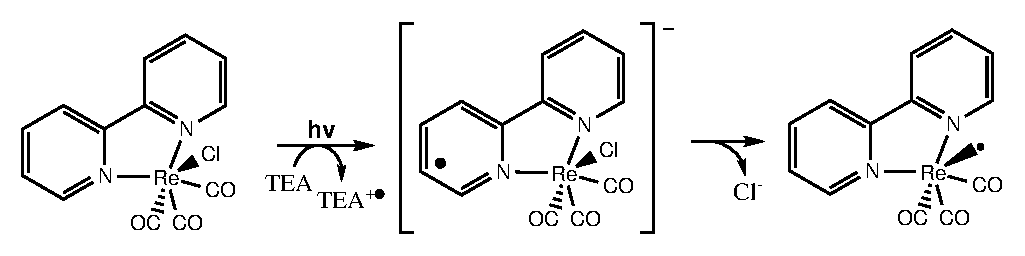
\includegraphics[clip=true, width=120mm, keepaspectratio]{images/eximer.eps}
 \end{center}
\caption{Formation of the eximer species via absorption of a photon and oxidation of the sacrificial amine.}
\label{fig.eximer}
\end{figure} 

The decomposition route of the sacrificial amine was first identified by Kalyansundarem in 1978\autocite{kalyanasundaram1978}, and is summarized in \autoref{fig.decomp}. This work showed the decomposition of \gls{ac.teoa} but the mechanism for decomposition of \gls{ac.tea} is parallel. This decomposition is critical due to the protons it provides to the reaction mixture, and the presence of a simple second electron abstraction from the decomposition product. Upon absorption of a photon by the catalyst, the amine \textbf{4.05} is converted to the radical cationic species (\ce{Et3N+^{$\bullet$}}, \textbf{4.06}). This undergoes a proton transfer to a second molecule of the sacrificial reductant. The transfer removes a proton from the carbon $\alpha$ to the central nitrogen, leaving it a neutral radical species (forming \textbf{4.07}). This is then able to react in the catalytic cycle to provide a second electron and form the ethene-diethylamino compound. Triethylammonia is produced as well (\textbf{4.08}), this is a proton source for the formate and water-gas shift mechanistic pathways. This step is slightly exothermic, with energy releases of 1~kcal/mol in gas phase, or nearly 3~kcal/mol in \gls{ac.dmf}.

\begin{figure}[!htb]
 \begin{center}
  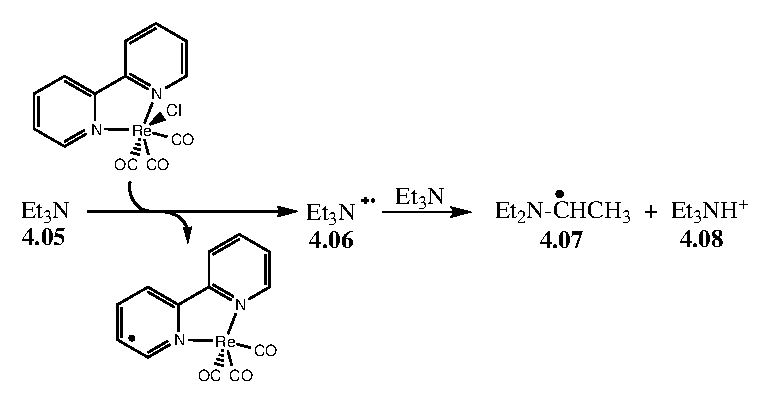
\includegraphics[clip=true, width=100mm, keepaspectratio]{images/reddecomp.eps}
 \end{center}
\caption{Decomposition pathway for the sacrificial amine.}
\label{fig.decomp}
\end{figure} 

Energies of \textbf{4.01} - \textbf{4.10}, and \textbf{4.26} in gas and solution phases (in \gls{ac.dmf}) is shown in \autoref{tab.supenergy}, along with the energy of solvation. Energies of each step of the reaction are listed in \autoref{tab.suprxn}. The values show a significant `uphill' series of steps requiring significant energy input. This energy is supplied by the incident photons; this process is a photocatalyzed activation. The reaction typically requires incident light of 400 nm\autocite{hawecker1983}, this high energy input allows for the excitation pathway to be followed.

% Table generated by Excel2LaTeX
\begin{table}[!htb]
\centering
 \begin{threeparttable}
  \caption[Gas phase and solvated energies for mechanism reactants and products]{Gas phase and solvated energies of mechanism reactants and products.}
    \begin{tabular}{llrrr}
    \toprule
    Molecule & Label & E (gas)\tnote{a} & E (solution)\tnote{b} & E (solvation)\tnote{c} \\
    \midrule
    Ground State & \textbf{4.01} & -1374.621419 & -1374.651099 & 18.62 \\
    3MLCT Complex & textbf{\textsuperscript{3}4.01\textsuperscript{MLCT}} & -1374.553193 & -1374.565998 & 8.04 \\
    Radical Anion & \textbf{4.02} & -1374.684002 & -1374.759190 & 47.18 \\
    Open Site Excimer & \textbf{4.03} & -914.3139376 & -914.3287245 & 9.28 \\
    Chlorine Anion & \textbf{4.04} & -460.2890817 & -460.4058583 & 73.28 \\
    Triethylamine (TEA) & \textbf{4.05} & -292.3051496 & -292.3854033 & 50.36 \\
    Radical Cation TEA & \textbf{4.06} & -292.3051496 & -292.3854033 & 50.36 \\
    Deprotonated TEA Radical & \textbf{4.07} & -291.9173706 & -291.9211226 & 2.35 \\
    Triethylammonia & \textbf{4.08} & -292.9552538 & -293.0382729 & 52.09 \\
    Carbon Dioxide & \textbf{4.09} & -188.6945676 & -188.6974631 & 1.82 \\
    Carbon Monoxide & \textbf{4.10} & -113.3744946 & -113.3754466 & 0.60 \\
    Diethylaminoethene & \textbf{4.26} & -291.3467768 & -291.3525868 & 3.64 \\
    \bottomrule
    \end{tabular}%
    \begin{tablenotes}
    \item [a] TPSS energy in hartrees.
    \item [b] TPSS energy in hartrees with COSMO solvation in DMF.
    \item [c] TPSS solvation energy in kcal/mol (E(gas) - E(solution)).
    \end{tablenotes}
  \label{tab.supenergy}%
 \end{threeparttable}
\end{table}%



% Table generated by Excel2LaTeX
\begin{table}[!htb]
\centering
 \begin{threeparttable}
  \caption{Energies for the reaction steps in the photoinduced excimer formation pathway}
    \begin{tabular}{r@{ $\rightarrow$ }lrr}
    \toprule
    \multicolumn{2}{c}{Steps} & Energy(gas)\tnote{a} & Energy(dmf)\tnote{b} \\
    \midrule
    \textbf{4.01} & \textbf{\textsuperscript{3}4.01\textsuperscript{MLCT}} & 42.81 & 53.40 \\
    \textbf{4.01\textsuperscript{3MLCT}} + \textbf{4.05} & \textbf{4.02} + \textbf{4.06} & 81.45 & -5.80 \\
    \textbf{4.02} & \textbf{4.03} + \textbf{4.04} & 50.82 & 15.44 \\
    \textbf{4.06} + \textbf{4.05} & \textbf{4.07} + \textbf{4.08} & -1.08 & -2.92 \\
    \bottomrule
    \end{tabular}%
    \begin{tablenotes}
    \item [a] TPSS energy in kcal/mol.
    \item [b] TPSS energy in kcal/mol with COSMO solvation in DMF.
    \end{tablenotes}
  \label{tab.suprxn}%
 \end{threeparttable}
\end{table}%




Geometries of the catalyst do not change significantly throughout this transformation, however, some small changes occur signifying the change in electron localization. One metric analyzed in polyaromatic non-innocent ligand redox reactions is the bonding distance between aromatic rings \autocite{bokarev2014}. From ground state, through triplet MLCT complex to the excited radical, the C-C\textsubscript{(bpy)} distance decreases from 1.470~\r{A} to 1.425~\r{A}, ending at 1.416~\r{A}. This 0.06~\r{A} decrease is noted in many previous experiments and calculations for anion radicals\autocite{bokarev2014, chisholm1981, castellaventura2000, gorerandall2009, irwin2010}. Other key bond lengths and angles include the ligand N-Re bonds and \ce{CO}-Re bonds, the addition and subtraction of electrons to and from the complex impact the bonding. As the reaction proceeds, for example, the calculated Re-N distance in solvated structures decreases from 2.18924~\r{A} in the ground state catalyst to 2.14212~\r{A} in the neutral radical excimer. Similarly, the distance from the metal to the axial carbonyl decreases from 1.91950 to 1.88746~\r{A} in the same circumstances. These changes are not significant, the bond order is unchanged. Bond length changes of 0.05~\r{A} are large enough to demonstrate a change has occurred in the electron configuration around the metal centre. 

%---------------------------------------------------------------------
\subsection{The `Carbonate' Pathway}\label{ss.carbonate}
%---------------------------------------------------------------------

The carbonate pathway is shown in \autoref{fig.carbonate}, starting from the excimer species. This pathway has been studied in some detail in the literature, but never as completely as will be shown here. Typical analysis consists of investigation from the formed \ce{CO2} linked dimer, through the release of \ce{CO}, terminating at the bicarbonate linked dimer. Studies typically build the dimer as a three-body reaction, or start with a \ce{Re\bond{-}Re} bound catalyst dimer and the insertion of \ce{CO2}. However, the formation of the  \ce{[L2Re(CO)3]2} is exceptionally slow in the presence of solvent, with a rate constant 8 orders of magnitude below the solvent-stabilized radical \ce{$^\bullet$L2Re(CO)3(solv)} complex\autocite{fujita2004}. 

\begin{figure}[!ht]
 \begin{center}
  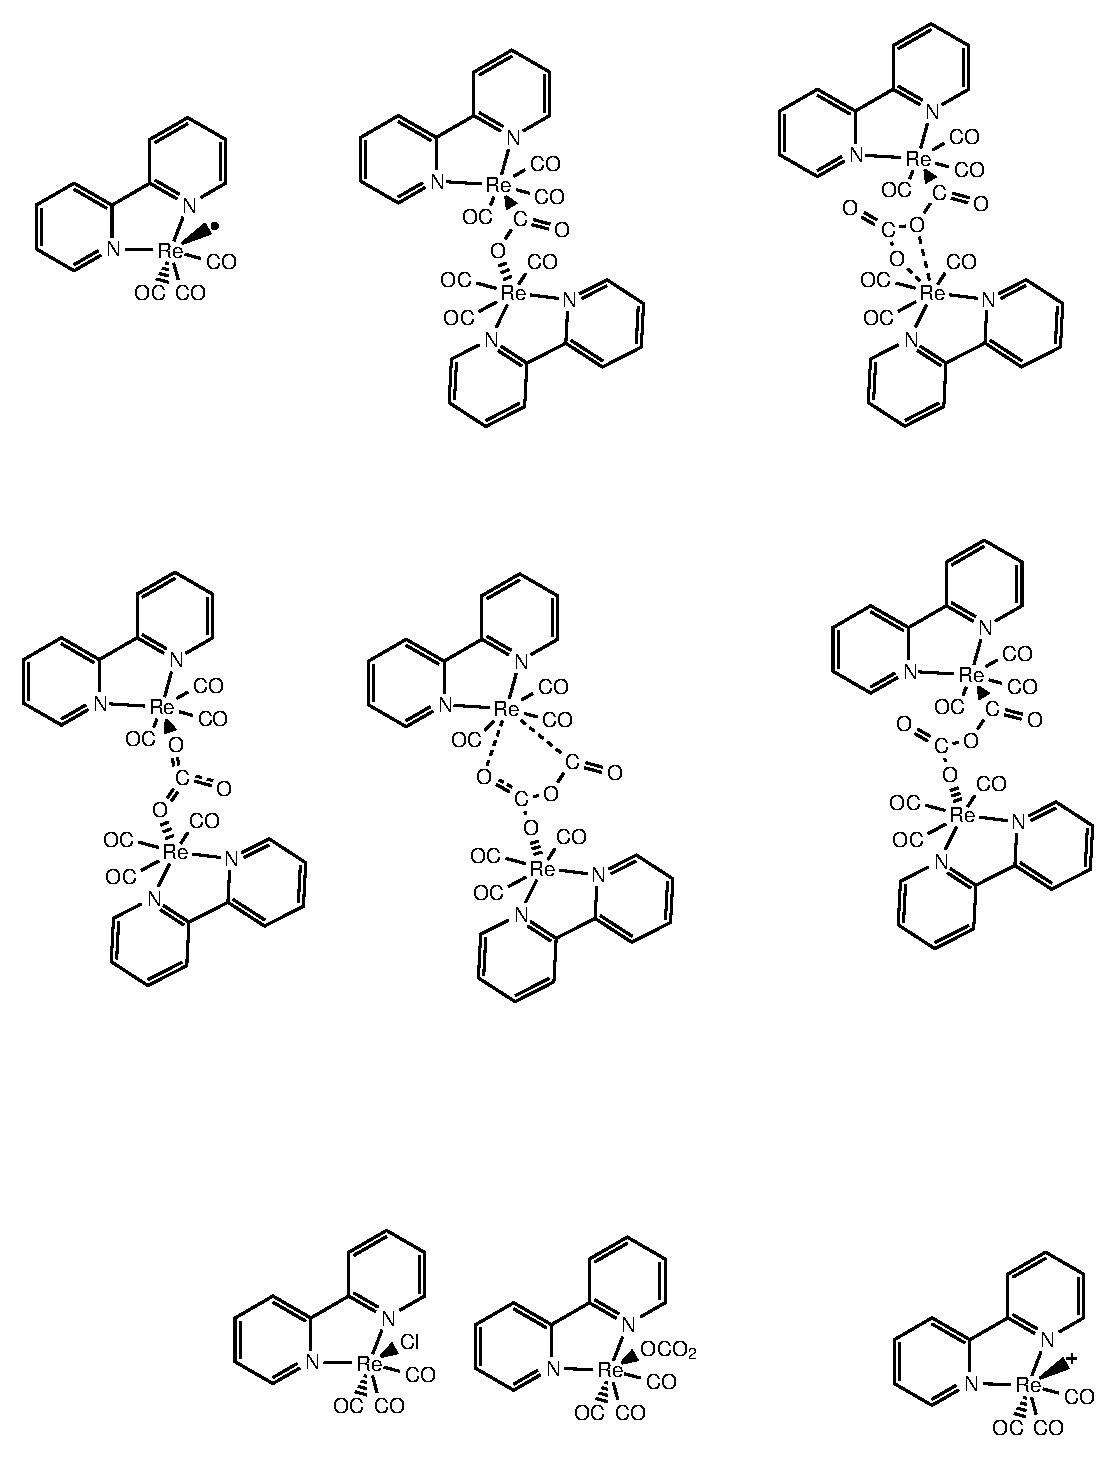
\includegraphics[clip=true, width=140mm, keepaspectratio]{images/carbonate.eps}
 \end{center}
\caption{The `carbonate' mechanistic pathway}
\label{fig.carbonate}
\end{figure} 

\Gls{ac.dft} energies of each of the compounds involved in this mechanism pathway are shown in \autoref{tab.carbenergy}, along with the energy of solvation. \autoref{tab.carbrxn} shows the potential energy change in each step of the reaction. The computed intermediate and transition state structures are shown in \autoref{fig.carbonatestruc}.

% Table generated by Excel2LaTeX
\begin{table}[!htb]
\centering
 \begin{threeparttable}
  \caption[Gas phase and solvated energies for the `carbonate' mechanism]{Gas phase and solvated energies of compounds, transition states and intermediates in the `carbonate' mechanism}
    \begin{tabular}{llrrr}
    \toprule
    Molecule & Label & E (gas)\tnote{a} & E (solution)\tnote{b} & E (solvation)\tnote{c} \\
    \midrule
    \ce{CO2} Linked Dimer & 4.11 & -2017.373132 & -2017.412314 & 24.59 \\
    \ce{CO2} Addition TS & 4.12 & -2206.120721 & -2206.165017 & 27.80 \\
    \ce{C2O4} Linked Dimer & 4.13 & -2206.047558 & -2206.097328 & 31.23 \\
    5 Member Ringed Dimer TS & 4.14 & -2206.013925 & -2206.061531 & 29.87 \\
    \ce{CO3} Linked Dimer & 4.15 & -2092.678255 & -2092.725669 & 29.75 \\
    Bicarbonate Catalyst Cation & 4.16 & -1178.065153 & -1178.119717 & 34.24 \\
    Bicarbonate Anion & 4.17 & -264.4852375 & -264.4967144 & 7.20 \\
    Dimer Formation TS & 4.18 & -2017.434125 & -2017.47423151664 & 25.17 \\
    Bicarbonate Dianion & 4.19 & -263.7946209 & -264.1983931 & 253.37 \\
    Open Site Cation & 4.27 & -914.1064097 & -914.1872844 & 50.75 \\
    \bottomrule
    \end{tabular}%
    \begin{tablenotes}
    \item [a] TPSS SCF energy in hartrees.
    \item [b] TPSS SCF energy in hartrees with COSMO solvation in DMF.
    \item [c] TPSS solvation energy in kcal/mol (E(gas) - E(solution)).
    \end{tablenotes}
  \label{tab.carbenergy}%
 \end{threeparttable}
\end{table}%



% Table generated by Excel2LaTeX
\begin{table}[!htb]
\centering
 \begin{threeparttable}
  \caption{Energies for the reaction steps in the `formate' pathway}
    % Table generated by Excel2LaTeX from sheet 'Tex Charts
    \begin{tabular}{rrrr}
    \toprule
    Description & Steps & Energy(gas)\tnote{a} & Energy(dmf)\tnote{b} \\
    \midrule
    Formation of Radical Anion & 4.01, 4.05 \ce{->} 4.02, 4.06   & 124.261582 & 47.596907 \\
    Open site catalyst plus cl- & 4.02 \ce{->} 4.03, 4.04 & 50.816912 & 15.440887 \\
    Reconfiguration of TEA & 4.06, 4.05 \ce{->} 4.07, 4.08 & -1.077024 & -2.915901 \\
    \midrule
    Addition of CO2 to open site & 4.4   & -0.2501423 & 6.37310903 \\
    addition of second cat to CO2 & 4.5   & 118379.026 & 118375.044 \\
    Insertion of CO2 & 4.6   & \#VALUE! & -8.5491267 \\
    relaxation of co2 insertion & 4.7   & \#VALUE! & -0.6637971 \\
    rearrange to 4ring dimer & 4.8   & \#VALUE! & \#VALUE! \\
    relax to long & 4.9   & \#VALUE! & \#VALUE! \\
    rearrangement to 5ring dimer & 4.1   & \#VALUE! & 22.4628711 \\
    relax to final & 4.11  & \#VALUE! & -24.839557 \\
    break apart & 4.12  & 317.951051 & 262.714812 \\
    return to ground states & 4.13  & -613.91666 & -426.82371 \\
    \bottomrule
    \end{tabular}%
    \begin{tablenotes}
    \item [a] TPSS SCF energy in kcal/mol.
    \item [b] TPSS SCF energy in kcal/mol with COSMO solvation in DMF.
    \end{tablenotes}
  \label{tab.carbrxn}%
 \end{threeparttable}
\end{table}%


The mechanism begins with the addition of a \ce{CO2} molecule to the excimer \textbf{4.03}, forming \textbf{4.11}. This is a very weakly bound species when solved in a simulated \gls{ac.dmf} environment; in the gas phase this transition complex will not solve. Energies for the gas phase for this compound are calculated as single point energies from the solvated structure. The \gls{ac.dmf} solved structure has a Re-C bond length of 2.50654~\r{A}, and O-C-O bonding angle of 142$^\circ$, when compared to the \ce{Re\bond{-}C} distances of rhenium carbonyls of \textit{ca}. 1.9~\r{A}, this is a very weak bond. The formation of this complex requires only 6.37~kcal/mol, the radical species is not satisfied with the addition of \ce{CO2} and requires further electron contribution to become more stable. This unstable complex is able to extract a hydrogen from triethylammonia (\ce{Et3NH+}, \textbf{4.08}) to continue with the `water-gas' pathway (see below \autoref{ss.watergas}), or combine with a second molecule of the excimer to form a dimer \textbf{4.12}. This dimer formation is favourable; resolution of radical species is provided. The addition of the second catalyst releases42.5~kcal/mol in \gls{ac.dmf}. The quenching of the radical forms much stronger bonds between the metal atoms and the linking \ce{CO2}. The Re-C distance has shortened from the 2.50654~\r{A} seen in \textbf{4.11} to 2.25829~\r{A}. This is still longer than the Re-CO bonds, which is expected due to the lack of $\pi$ back-bonding observed with carbonyl ligands, however, it corresponds with similar published crystal structures of Re-C bond lengths for sp\textsuperscript{2} carbons\autocite{lukehart1977}. The Re-O bond is 2.13~\r{A}, a value that remains constant for Re-O through the intermediates in the reaction pathway.

\begin{figure}[!ht]
 \begin{center}
  \includegraphics[clip=true, width=120mm, keepaspectratio]{images/carbonatestruc.eps}
 \end{center}
\caption{DFT calculated structures for the `carbonate' mechanistic pathway}
\label{fig.carbonatestruc}
\end{figure} 

After the dimer \textbf{4.12} has been formed, a second molecule of \ce{CO2} is inserted via transition state \textbf{4.13} to form the Re-C-O-C-O-Re complex \textbf{4.14} (see structures \textbf{4.11} - \textbf{4.17}\todo{fix after image made} in \autoref{fig.carbonatestruc}). This linker contains bonds from length 1.28~-~1.44~\r{A}, typical for sp\textsuperscript{2}-carbon oxygen bonds\todo{Ref CRC Handbook}. Bond angles are typically just under the idealized 120$^\circ$ expected as well. Due to the linker, the two catalyst ligand bipyridines have moved from a nearly co-planar geometry to a nearly perpendicular geometry. Re-C and Re-O bonds remain constant in length compared to \textbf{4.12}. The formation of a 5 membered ring transition state structure \textbf{4.15} costs 22~kcal/mol. This leads to the release of the \ce{CO} and the formation of a carbonate linked dimer, \textbf{4.16}, resulting in a net energy decrease of -2.4~kcal/mol, and returning the catalyst ligands to a more co-planar orientation. The carbonate dimer species is left to decompose to a catalyst cation \textbf{4.19}\todo{?} with an open site, and the bicarbonate adduct \textbf{4.17}. This carbonate dianion may pick up a proton before or after the disassociation to the catalyst cationic species, resulting in the released of the bicarbonate species to solution (\textbf{4.18)} when the catalyst is returned to ground state \textbf{4.01} with addition of a chloride. The decomposition of the bicarbonate dimer species has a barrier of 262~kcal/mol in \gls{ac.dmf}. This is due to the charge separations that occur, while solvation stabilizes these charged species it does not accurately simulate a system with an ionic strength similar to what could be expected in the experimental reaction. The Gibbs energy for this step was calculated to be -11.4~kcal/mol in solution, with an additional -17~kcal/mol for the anion exchange, signifying the thermodynamic favourableness of this transformation. The presence of excess molar equivalents of an electrolyte such as tetraethylammoniumchloride ensures a surplus of chloride anions are in solution and are an additional force for conversion, according to Le Ch\^{a}telier's principle.

%---------------------------------------------------------------------
\subsection{The `Formate' Pathway}\label{ss.formate}
%---------------------------------------------------------------------
In comparison to the catalytic dimer formed in the carbonate pathway above, the formate formation occurs via a much simpler mechanism. The addition of a hydrogen to the open site axial to the ligand occurs via the simultaneous electron and proton transfer from a by-product of the reduction of the amine. \ce{CO2} inserts into this metal hydride bond, resulting in a metal-oxide bond, with the formate anion\autocite{creutz2007}. Separation of the weak metal-oxygen bond allows for the reinsertion of the halide to the cationic metal centre. 

\begin{figure}[!htb]
 \begin{center}
  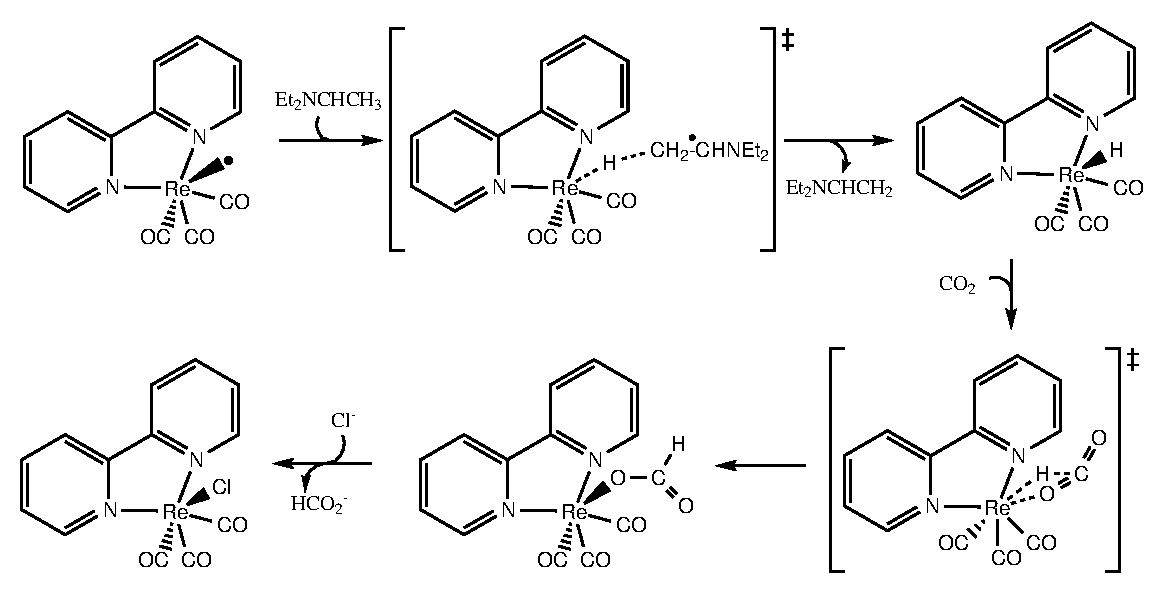
\includegraphics[clip=true, width=\textwidth, keepaspectratio]{images/formate.eps}
 \end{center}
\caption{The `formate' mechanistic pathway}
\label{fig.formate}
\end{figure} 

\Gls{ac.dft} energies of each of the compounds involved in this mechanism pathway are shown in \autoref{tab.formenergy}, along with the energy of solvation. \autoref{tab.formrxn} shows the potential energy change in each step of the reaction. The computed intermediate and transition state structures are shown in \autoref{fig.formatestruc}.

% Table generated by Excel2LaTeX
\begin{table}[!htb]
\centering
 \begin{threeparttable}
  \caption[Gas phase and solvated energies for the `formate' mechanism]{Gas phase and solvated energies of compounds, transition states and intermediates in the `formate' mechanism}
    \begin{tabular}{llrrr}
    \toprule
    Molecule & Label & E (gas)\tnote{a} & E (solution)\tnote{b} & E (solvation)\tnote{c} \\
    \midrule
    Proton Transfer TS & 4.21  & -1206.302997 & -1206.32707 & 15.10 \\
    Catalyst Hydride & 4.22  & -914.9204746 & -914.9448354 & 15.29 \\
    \ce{CO2} Insertion TS & 4.23  & -1103.581201 & -1103.619960 & 24.32 \\
    Catalyst Formate & 4.24  & -1103.635283 & -1103.665628 & 19.04 \\
    Formate Anion & 4.25 & -189.3051464 & -189.4151284 & 69.01 \\
    Open Site Cation & 4.27  & -914.1064097 & -914.1872844 & 50.75 \\
    \bottomrule
    \end{tabular}%
    \begin{tablenotes}
    \item [a] TPSS SCF energy in hartrees.
    \item [b] TPSS SCF energy in hartrees with COSMO solvation in DMF.
    \item [c] TPSS solvation energy in kcal/mol (E(gas) - E(solution)).
    \end{tablenotes}
  \label{tab.formenergy}%
 \end{threeparttable}
\end{table}%



% Table generated by Excel2LaTeX
\begin{table}[!htb]
\centering
 \begin{threeparttable}
  \caption{Energies for the reaction steps in the `formate' pathway}
    % Table generated by Excel2LaTeX from sheet 'Tex Charts
    \begin{tabular}{rrrr}
    \toprule
    Description & Steps & Energy(gas)\tnote{a} & Energy(dmf)\tnote{b} \\
    \midrule
    Formation of Radical Anion & 1.1   & -39.271301 & -67.827267 \\
    Open site catalyst plus cl- & 1.2   & 50.8169125 & 15.4408871 \\
    Reconfiguration of TEA & 1.3   & -164.60991 & -118.34007 \\
    \midrule
    Hydride Extraction & 1.4   & 4.09794743 & -9.8319638 \\
    Removal of TEA & 1.5   & -26.652434 & -20.021496 \\
    Insertion of CO2 & 1.6   & 21.2356096 & 14.0177223 \\
    recoordination & 1.7   & -33.936535 & -28.657394 \\
    dissasotiation of HCO2- & 1.8   & 140.389052 & 39.6680755 \\
    Reformation of Catalyst & 1.9   & -141.76995 & -36.367745 \\
    \bottomrule
    \end{tabular}%
    \begin{tablenotes}
    \item [a] TPSS SCF energy in kcal/mol.
    \item [b] TPSS SCF energy in kcal/mol with COSMO solvation in DMF.
    \end{tablenotes}
  \label{tab.formrxn}%
 \end{threeparttable}
\end{table}%



After formation of the excimer \textbf{4.03}, the radical species extracts a hydrogen atom from the oxidized chain of the sacrificial amine \textbf{4.07} in transition state \textbf{4.21}, a step releasing 45~kcal/mol in the gas phase or 48.5~kcal/mol in \gls{ac.dmf}. This is due to the satisfaction of the radical states and removal of the charge on the amine. The sacrificial amine involved in this step had previously had one proton extracted by another molecule of the amine in a proton exchange step (see \autoref{ss.initiation}), resulting in a neutral radical. Extraction of the proton and electron pair allows for the formation of the ethene, completing the decomposition of the amine to the final neutral, singlet molecule \textbf{4.26}. Relaxation of this transition state results in the hydrogen extraction from the radical species, yielding the formation of the hydride complex \textbf{4.22}.

\begin{figure}[!ht]
 \begin{center}
  
\includegraphics[clip=true, width=120mm, height=70mm, keepaspectratio]{images/insertgraphic.eps}
 \end{center}
\caption{DFT calculated structures for the `formate' mechanistic pathway}
\label{fig.formatestruc}
\end{figure} 

This hydride complex is able to insert a molecule of \ce{CO2} into the metal-hydrogen bond, in transition step \textbf{4.23}, with only a 14.4~kcal/mol barrier to transition state formation.. \ce{CO2} insertion to metal hydrides is commonly observed, most mechanisms in \ce{CO2} reduction in similar ruthenium systems employ this addition\autocite{creutz2007}. The Re-H bond length is 1.76~\r{A}, compared to the length of the Re-Cl bond from the ground state \textbf{4.01} species of 2.51~\r{A}. This bond length difference reflects the observations on anion change from Cl to Br (as discussed in \autoref{chap.newchem}, \autoref{ss.xray}), the anion size is the critical factor in this variation. When a molecule of \ce{CO2} approaches, the transition state of a pseudo-septacoordinate species \textbf{4.23} forms. The Re-H bond increases in length to 2.16~\r{A}, the Re-O bond is 2.88~\r{A}, and the O-Re-H angle is very tight, at only 45.3$^\circ$. This step completes with 28.66~kcal/mol energy release to form the formato anion complex \textbf{4.24}. 

The formato anion \textbf{4.24} contains a Re-O bond of 2.15~\r{A}, consistent with previously discussed rhenium - oxygen bonds. This formate dissociates with a chloride addition, the exchange is endothermic by less than 3~kcal/mol overall, but has a barrier of nearly 40~kcal/mol in DMF (or 140~kcal/mol in gas phase) calculations. As discussed with the carbonate mechanism, this large barrier is due to the charge separation that occurs. The calculated Gibbs energy for the formation of the charge separated transition state is -12.7~kcal/mol in solvent, showing the thermodynamic favourableness of this exchange. Further reactions of the formato anion in solution are not investigated, but the anion may remain deprotonated in the slightly basic environment\autocite{morimoto2013}. 

Some attempts were made at performing the reaction along alternative pathways. While direct $\sigma$ bonding from a metal to an oxygen atom in the \ce{CO2} molecule (as $\eta^1$-OCO) has been observed in a few systems (including photoreduction of \ce{CO2} on other metal systems)\autocite{lee2001, mauser2001, souter1997}, this geometry is rare\autocite{castrorodriguez2004, cokoja2011, gibson1996}. Attempts to coordinate \ce{CO2} in an $\eta^1$-OCO geometry failed to converge both in gas and solution phase, as \ce{CO2} was ejected from the complexBinding of \ce{CO2} to the metal through $\pi$ coordination of the C=O bond is more common\autocite{cokoja2011, gibson1996}, but these structures failed to solve in the current \gls{ac.dft} system as well, typically via the dissociation of the \ce{CO2}.

\FloatBarrier

%---------------------------------------------------------------------
\subsection{The `Water-Gas Shift' Pathway}\label{ss.watergas}
%---------------------------------------------------------------------
The water-gas shift mechanism involves the addition of two protons from the reductant to a \ce{CO2} molecule bound to the metal centre. The first proton addition yields an acid species, this is dehydrated via the second addition of a proton and the release of one molecule of \ce{H2O}. The resulting tetracarbonyl cationic species is able then to release an axial carbonyl to return to the ground state. While any of the carbonyl groups could be labile, the carbonyl at the axial position is the one actively replaced by the halide to return to the starting catalyst\autocite{shaver1992}. 

\begin{figure}[!htb]
 \begin{center}
  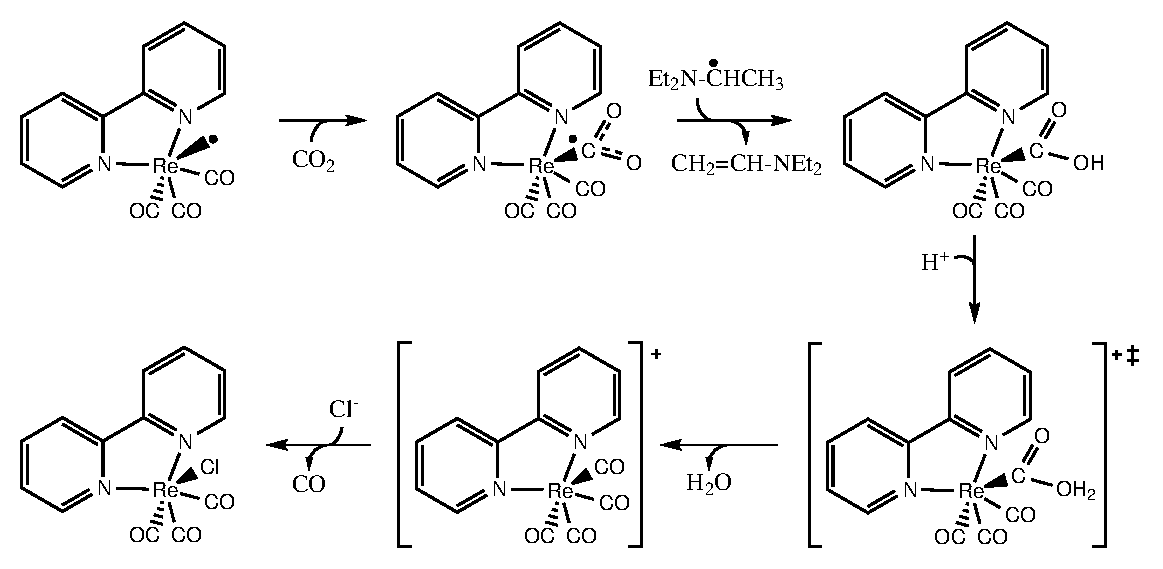
\includegraphics[clip=true, width=\textwidth, keepaspectratio]{images/watergas.eps}
 \end{center}
\caption{The `water-gas shift' mechanistic pathway}
\label{fig.watergas}
\end{figure} 

\Gls{ac.dft} energies of each of the compounds involved in this mechanism pathway are shown in \autoref{tab.wgsenergy}, along with the energy of solvation. \autoref{tab.wgsrxn} shows the potential energy change in each step of the reaction. The computed intermediate and transition state structures are shown in \autoref{fig.wgsstruc}.

% Table generated by Excel2LaTeX
\begin{table}[!htb]
\centering
 \begin{threeparttable}
  \caption[Gas phase and solvated energies for the `water-gas shift' mechanism]{Gas phase and solvated energies of compounds, transition states and intermediates in the `water-gas shift' mechanism}
    \begin{tabular}{llrrr}
    \toprule
    Molecule & Label & E (gas)\tnote{a} & E (solution)\tnote{b} & E (solvation)\tnote{c} \\
    \midrule
    Catalyst-\ce{CO2} (Axial) & 4.31  & -1103.008904 & -1103.016031 & 4.47 \\
    Catalyst-\ce{CO2H} (Axial) & 4.32  & -1103.610331 & -1103.640451 & 18.90 \\
    \ce{H2O} Dissociation (Axial) TS & 4.33  & -1104.018352 & -1104.093313 & 47.04 \\
    Catalyst-\ce{CO2} (Equatorial) & 4.34  & -1102.963633 & -1102.992198 & 17.92 \\
    Catalyst-\ce{CO2H} (Equatorial) & 4.35  & -1103.597572 & -1103.625739 & 17.68 \\
    \ce{H2O} Dissociation (Equatorial) TS & 4.36  & -1104.016156 & -1104.093644 & 48.62 \\
    Water & 4.37 & -76.46413339 & -76.47581393 & 7.33 \\
    Tetracarbonyl Catalyst Cation & 4.38  & -1027.546073 & -1027.619412 & 46.02 \\
    H Transfer to Axial \ce{CO2} TS & 4.39  & -1394.981543 & -1395.011603 & 18.86 \\
    H Transfer to Equatorial \ce{CO2} TS & 4.40  & -1394.938949 & -1394.991623 & 33.05 \\
    Catalyst with Migrated Open Site & 4.41  & -914.2766988 & -914.2972247 & 12.88 \\
    \bottomrule
    \end{tabular}%
    \begin{tablenotes}
    \item [a] TPSS SCF energy in hartrees.
    \item [b] TPSS SCF energy in hartrees with COSMO solvation in DMF.
    \item [c] TPSS solvation energy in kcal/mol (E(gas) - E(solution)).
    \end{tablenotes}
  \label{tab.wgsenergy}%
 \end{threeparttable}
\end{table}%



% Table generated by Excel2LaTeX
\begin{table}[!htb]
\centering
 \begin{threeparttable}
  \caption{Energies for the reaction steps in the `formate' pathway}
    \begin{tabular}{rrrr}
    \toprule
    Description & Steps & Energy(gas)\tnote{a} & Energy(dmf)\tnote{b} \\
    \midrule
    Formation of Radical Anion & 2.1   & -39.271301 & -67.827267 \\
    Open site catalyst plus cl- & 2.2   & 50.8169125 & 15.4408871 \\
    Reconfiguration of TEA & 2.3   & -164.60991 & -118.34007 \\
    \midrule
    migration of open site? & 2.4   & 23.3674263 & 19.7662463 \\
    Addition of CO2 to open site & 2.5   & 4.78987184 & 1.56207334 \\
    H transfer to CO2 & 2.6   & -61.998066 & -35.596525 \\
    CO2H planar relaxation & 2.7   & 22.2489536 & -5.1943905 \\
    COOH2 ts & 2.8   & 144.908364 & 116.570584 \\
    CO4 + and water & 2.9   & 4.10436095 & -1.4970678 \\
    dissassotiation of CO & 2.10  & 40.893777 & 35.5673996 \\
    Reformation of Catalyst & 2.11  & -141.76995 & -36.367745 \\
    \bottomrule
    \end{tabular}%
    \begin{tablenotes}
    \item [a] TPSS SCF energy in kcal/mol.
    \item [b] TPSS SCF energy in kcal/mol with COSMO solvation in DMF.
    \end{tablenotes}
  \label{tab.wgsrxn}%
 \end{threeparttable}
\end{table}%




This mechanistic pathway it thought to start by the same addition of \ce{CO2} that is seen in the carbonate mechanism (see \autoref{ss.carbonate}), forming \textbf{4.11}. As before, the complex is only weakly coordinated, and requires solvation effects to solve computationally. The added \ce{CO2} is able to extract a hydrogen from the previously-reduced sacrificial amine \textbf{4.07} with a net energy change of -35.1~kcal/mol in \gls{ac.dmf}, again allowing the formation of the ethene amine \textbf{4.26}. The newly formed acid species \textbf{4.32} dehydrates in the presence of a second proton (via \textbf{4.33}) to form water \textbf{4.37} and the tetracarbonyl cationic species \textbf{4.38}. This has an energy cost of 9~kcal/mol in solution, but the $\Delta$G is -15~kcal/mol. This tetracarbonyl cation exchanges a \ce{CO} molecule for a \ce{Cl-} to return to \textbf{4.01}, with a 0.8~kcal/mol energy release.

\begin{figure}[!ht]
 \begin{center}
  
\includegraphics[clip=true, width=120mm, height=70mm, keepaspectratio]{images/insertgraphic.eps}
 \end{center}
\caption{DFT calculated structures for the `water-gas shift' mechanistic pathway}
\label{fig.wgsstruc}
\end{figure} 

Typically, this reaction had been thought to proceed on the axial site of the catalyst, mirroring the pathways discussed above. However, due to the ease of migration of carbonyl groups in organometallic complexes, it is proposed that the `water-gas shift' mechanism does not occur axial to the ligand, but begins with relocation of a \ce{CO2} ligand to the axial position, followed by the coordination of \ce{CO2} into the now vacant planar open site, forming \textbf{4.34} (energies for this reaction are shown in \autoref{tab.siderxn}). This \ce{CO2} bound in the plane of the ligand then undergoes hydrogen addition and dehydration to produce a molecule of \ce{H2O}, continuing as before. Once reduced to the tetracarbonyl cluster, the catalyst could shed any \ce{CO} ligand and pick up a chloride anion to return to the neutral ground state. However, labilization of the axial carbonyl is the most favoured, formation of the planar coordinated chloride complex is not expected\autocite{shaver1992}

% Table generated by Excel2LaTeX
\begin{table}[!htb]
\centering
 \begin{threeparttable}
  \caption{Energies for the reaction steps in the `formate' pathway}
    % Table generated by Excel2LaTeX from sheet 'Tex Charts
    \begin{tabular}{rrrr}
    \toprule
    Description & Steps & Energy(gas)\tnote{a} & Energy(dmf)\tnote{b} \\
    \midrule
    Formation of Radical Anion & 4.01, 4.05 \ce{->} 4.02, 4.06   & 124.261582 & 47.596907 \\
    Open site catalyst plus cl- & 4.02 \ce{->} 4.03, 4.04 & 50.816912 & 15.440887 \\
    Reconfiguration of TEA & 4.06, 4.05 \ce{->} 4.07, 4.08 & -1.077024 & -2.915901 \\
    \midrule
    Addition of CO2 to open site & 3.4   & -0.2501423 & 6.37310903 \\
    H transfer to CO2 & 3.5   & -19.133571 & -33.878805 \\
    CO2H axial relaxation & 3.6   & -0.2145456 & -1.1883574 \\
    COOH2 ts & 3.7   & 151.907871 & 125.579781 \\
    CO4 + and water & 3.8   & 5.1112987 & -1.2748062 \\
    dissassotiation of CO & 3.9   & 40.893777 & 35.5673996 \\
    Reformation of Catalyst & 3.10  & -141.76995 & -36.367745 \\
    \bottomrule
    \end{tabular}%
    \begin{tablenotes}
    \item [a] TPSS SCF energy in kcal/mol.
    \item [b] TPSS SCF energy in kcal/mol with COSMO solvation in DMF.
    \end{tablenotes}
  \label{tab.siderxn}%
 \end{threeparttable}
\end{table}%




This newly proposed mechanism provides a solution to a previously unexplained phenomenon. The exchange of carbonyl groups on the catalyst for \ce{^{13}CO} when using \ce{^{13}CO2} in the photoreduction is documented as early as Hawecker \textit{et al} in 1986\autocite{hawecker1986}. It was shown that complete exchange occurs with very few catalytic turnovers. Furthermore, Koike \textit{et al}. demonstrated that photochemical ligand substitution occurs at only axial sites relative to the $\alpha$-imino ligand\autocite{koike2002}, no exchange occurs at the equatorial site, nor can the \textit{fac}-\ce{(^{12}CO)2^{13}CO} be expected to shift the \ce{^{13}CO} to the equatorial position in the time-frame of the reaction. Thus the isotopic exchange does not proceed by independent uptake of produced \ce{^{13}CO}, but in fact the conversion to the \ce{^{13}CO} complex must be inherent to the reduction mechanism. 

This modified geometry does not violate any previously published experimental mechanism work. These studies typically focus on photophysical or spectroscopic analysis to determine intermediates, the analysis methods are not rigid geometry descriptors. Reevaluation of the spectral data within these newly defined parameters does not invalidate the work, mechanistic descriptors published (such as kinetics) are still valid within the new geometry.

As well, this provides an explanation for the lack of \ce{CO2} reduction by (terpy)-$\kappa^3$-\ce{Re(CO)3Cl} discussed in \autoref{chap.co2}. While the carbonyl group is transitioning to the axial site, before \ce{CO2} has been coordinated to the complex, the catalyst is available for chelation of the pendant arm (see \autoref{scheme.tricarbonyl}. 

\FloatBarrier

%---------------------------------------------------------------------
\subsection{Consequences From \texorpdfstring{\ce{$\kappa$^2}}{Bidentate} Terpyridine Complex Inactivity}
%---------------------------------------------------------------------

The \todo{maybe take this section out? covered in rationalization section ch3} lack of reactivity of the \ce{$\kappa$^2(terpy)Re(CO)3X} motif of complexes contrasting to the activity of the originally published \ce{$\kappa$^2(bipy)Re(CO)3X} indicates significant influence of the ligand on the mechanism. While the terdentate complex can be rationalized to be inactive due to its short-lived excited state (as seen in \autoref{chap.newchem}) \autocite{shavaleev2004}, this explanation does not suffice for the fluorescing bidentate complex. Other substituted bipyridine ligands are known to be active for photocatalytic reduction \autocite{hawecker1986, kurz2006}, identifying the most likely conflicting feature of the terpyridine ligand to be the pendant arm, and its availability for chelation to the metal centre. While in the radical eximer form, the chelation site is sterically blocked by one of the three carbonyl groups. However, reorganization of the substituent carbonyls from a \textit{facial} orientation to a \textit{meridional} could allow for the free pyridine to form the metal-ligand bond, resulting in compound \textbf{3.1} (see \autoref{chap.co2}, \autoref{ss.rationalization}).

%======================================================================
\section{Comparison Between Mechanistic Pathways} \label{sec.compare}
%======================================================================

Previous studies in literature had only analyzed one of the mechanistic pathways (or a subsection thereof), without a fuller analysis of the competitiveness of each pathway relative to the others. Discussion on the tenability of each potential pathway relied on the \textit{in situ} observation of intermediates or transition states, the success (or lack thereof) of synthesis of the intermediates, and the relative production of by-products in the mechanistic trials. 

The overall energies for each of the mechanistic pathways shown in \autoref{fig.threepath} are shown in \autoref{fig.threeenergies}. 

\begin{figure}[!htbp]
 \begin{center}
  
\includegraphics[clip=true]{images/insertgraphic.eps}
 \end{center}
\caption[Reaction energies for three mechanistic pathways]{An overview of the energies of the three mechanistic pathways of photochemical \ce{CO2} reduction}
\label{fig.threeenergies}
\end{figure} 
\todo{SOLVE ENERGY, make figure}

The comparison between mechanisms show the difficulty in determining the most likely reaction pathway based on computational analysis alone. Both the formate and water-gas routes have the maximum transition energy barrier for the final disassociation of the product and coordination of chloride. This barrier is artificially high, the charge separation that occurs is impacted significantly by the basic pH and the presence of electrolyte in solution experimentally. These factors are not taken into consideration in the calculations. Gibbs energies were calculated for these steps, the average $\Delta$G values are around -12~kcal/mol for the production of the transition state, signifying a thermodynamically favoured reaction. The overall energy of the exchange 

Due to the similarity in potential energy profiles for these reactions, analysis of experimental data must be undertaken to accurately predict which pathway dominates the photoreduction of \ce{CO2}. 

It's important to note that the energy requirements of each pathway is not the only indicator of mechanistic preference. Studies have shown the mechanism rate differs between pathways, with certain intermediates nearly blocking the progression of the redox reaction.

%======================================================================
\section{Conclusions} 
%======================================================================

With the energies of each of the independent mechanisms elucidated, the feasibility of each mechanism becomes evident. Evidence in literature suggests that all mechanisms progress to some degree, however, the production of \ce{CO} outpaces that of the partial reduction or oxidation pathways. 
